\section{Evaluation}
\label{sec:eval}

\figref{fig:bench} shows the results of a small experiment measuring the compile
 time of our implementation.
The code used the run the experiment and generate the figure is
 included in the appendix.

For each integer $N$ between 4 and 200 inclusive, we generated 20 random
 Kodkod programs and measured the time to complete a system call that invoked
 our compiler on the generated file.
Each green dot is the time for a single generated program.
The distribution is oddly bimodal, but even the worse trend is not bad\textemdash
 compile times run in less than 1 second and appear to scale linearly as programs
 grow in size.

To be precise, each $N$ generates a program with $N$ atoms, $N$ relational bounds,
 and $N$ binary formulas.
The lower and upper bounds for each relation are chosen randomly, but guaranteed to
 be syntactically valid.
The formulas are limited to binary relations for simplicity\textemdash each
 formula expresses a constraint on two of the relational variables.

As one might expect, less than $1\%$ of our generated formulas are satisfiable.
This is a threat to validity: non-trivial formulas may take much longer to compile.

Another point of note is that timings measure the real-time cost of a system
 call and I/O operation, both of which can be heavily affected by OS event regardless
 of the efficiency of our implementation.
Still, we chose this experiment to match the user experience of Kodkod $\sqrt{2}$.

\begin{figure}[t]
  \label{fig:bench}
  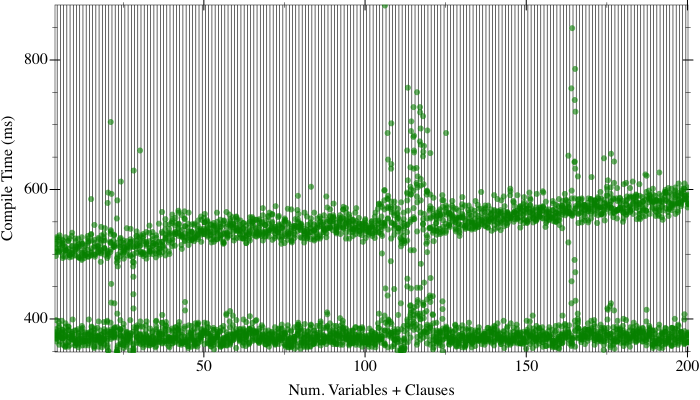
\includegraphics[width=10cm]{benchmark.png}
  \caption{Compile time vs. problem size}
\end{figure}

